En esta sección exploramos algunas características de el mercado en cuestión (Emisiónes de tarjetas crediticias por Fintechs), para así, conocer algunos aspectos relevantes a el proyecto en desarrollo.

\subsection*{Resumen Rappicard}
RappiCard ha emergido como un actor significativo en el mercado mexicano de tarjetas de crédito desde su lanzamiento en 2021. A continuación, se presentan datos clave que ilustran su crecimiento y posición en el sector:

\begin{itemize}
    \item \textbf{Cartera de crédito:} Para agosto de 2024, RappiCard alcanzó una cartera de crédito de 5,107 millones de pesos, consolidándose entre las fintech más destacadas del país~\cite{forbes_cartera_2024}.
    \item \textbf{Número de clientes:} En abril de 2024, la empresa superó el millón de clientes en México, reflejando una rápida adopción de sus servicios \cite{expansion_millon_2024}.
    \item \textbf{Líneas de crédito:} Gracias al análisis de datos de la plataforma Rappi, RappiCard ofrece líneas de crédito iniciales promedio de $18,000$ MXN, un 53\% superiores a las de otras fintechs \cite{chocale_millon_2024}.
    \item \textbf{Segmento demográfico:} Aproximadamente el 75\% de los clientes de RappiCard tienen menos de 35 años, indicando un enfoque exitoso en atraer a la población joven y digitalmente activa \cite{expansion_millon_2024}.
    \item \textbf{Proceso de aprobación y entrega:} RappiCard se distingue por su proceso ágil, con aprobaciones en dos minutos y entrega de la tarjeta física en un promedio de 30 minutos en áreas con cobertura de Rappi \cite{forbes_cartera_2024}.
    \item \textbf{Beneficios adicionales:} La tarjeta ofrece recompensas como 5\% de cashback en compras a través de RappiTravel y 1\% en otros comercios, además de no cobrar anualidad y permitir diferir compras mayores a $500$ MXN a meses sin intereses \cite{chocale_millon_2024}.
    \item \textbf{Índice de Morosidad (IMOR) de Banorte:} En el informe financiero del cuarto trimestre de 2023, se reportó un incremento en el índice de morosidad (IMOR) del segmento de tarjetas de crédito de Banorte, alcanzando el 3.3\%. Este aumento se atribuye a la consolidación de Banorte con RappiCard, ya que el IMOR era de 2.4\% en el mismo período del año anterior. El IMOR es una métrica clave en el análisis de riesgo crediticio, que mide el porcentaje de clientes que no han realizado pagos en sus tarjetas de crédito dentro de los plazos establecidos \cite{fintechexpertrappicardmorosidad}.
    \item \textbf{Visión de José Antonio Murillo, CEO de RappiCard:} En cuanto al futuro de la alianza entre RappiCard y Banorte, José Antonio Murillo comentó: “Hay mercado para todos”. Esta declaración refleja la confianza de RappiCard en su modelo de negocio y en la demanda de servicios digitales en el sector financiero, especialmente ante el auge de las fintechs como la propia RappiCard \cite{forbesrappibanorte}.
    \item \textbf{Modelo de operación digital de RappiCard:} El CEO de RappiCard también destacó que su modelo de operación digital, combinado con atención personalizada, ha sido un factor clave para su éxito. RappiCard ha logrado un Net Promoter Score (NPS) superior a los 80 puntos, comparado con el promedio de 37 puntos en la banca tradicional según encuestas de Banxico. Esto indica que los usuarios están muy satisfechos con el servicio y están dispuestos a recomendarlo, lo que refuerza su posición en el mercado \cite{forbesrappibanorte}.
    \item \textbf{Crecimiento de RappiCard:} Desde su lanzamiento en enero de 2021, RappiCard ha emitido más de 700,000 tarjetas de crédito y cuenta con un portafolio de crédito que supera los 4,000 millones de pesos. A tan solo dos años de su entrada al mercado, RappiCard ya ha superado en emisión de tarjetas a bancos internacionales establecidos desde hace décadas, lo que destaca su rápido crecimiento y aceptación~\cite{forbesrappibanorte}.
\end{itemize}

Estos indicadores reflejan el crecimiento acelerado y la sólida posición de RappiCard en el mercado financiero mexicano, especialmente entre los consumidores jóvenes y familiarizados con la tecnología.

\vspace{0.3cm}

\begin{itemize}
    \item El ecosistema fintech en México creció a una tasa del 18\% anual entre 2019 y 2023~\cite{dock2024}.
    \item Existen 844 startups fintech activas en el país~\cite{finnovating2024}.
    \item En 2023, las fintechs otorgaron más de 3,000 millones de dólares en préstamos, beneficiando a más de 5 millones de usuarios~\cite{uflow2024}.
    \item En 2021, solo el 32.7\% de la población entre 18 y 70 años tenía al menos un crédito formal~\cite{inegi2021}.
    \item Los ingresos del sector fintech crecieron a una tasa compuesta del 22\% anual entre 2021 y 2024, y 31\% en el último periodo (2023-2024)~\cite{reporteindigo2024}.
    \item El Índice de Maduración del Ecosistema Fintech (INFIN) se sitúa en 48\%, indicando una etapa de desarrollo aún temprana~\cite{santander2024}.
    \item Solo el 20\% de la población mexicana tiene una tarjeta de crédito; el efectivo sigue siendo el medio de pago principal~\cite{elfinanciero2024}.
\end{itemize}

En conjunto, estos indicadores reflejan un sector en plena transformación, con un impacto creciente en el acceso al crédito y la inclusión financiera en México.

\begin{figure}[h!]
    \centering
    \begin{subfigure}[b]{0.45\textwidth} % 'h!' for positioning
        \centering
        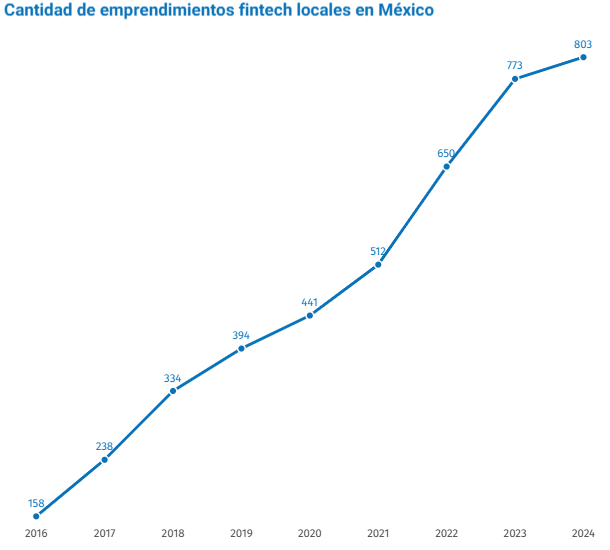
\includegraphics[scale=0.5]{Figuras/crecimientofintec.png} % scale the figure here
        \captionsetup{labelfont={color=white}, textfont={color=white}} % Cambia el color del caption
        \caption{Crecimiento de Fintechs.}
        \label{fig:crecfintechs}
    \end{subfigure}
    \hspace{0.005\textwidth} % Add some horizontal space between the subplots
    \begin{subfigure}[b]{0.45\textwidth} % 'h!' for positioning
        \centering
        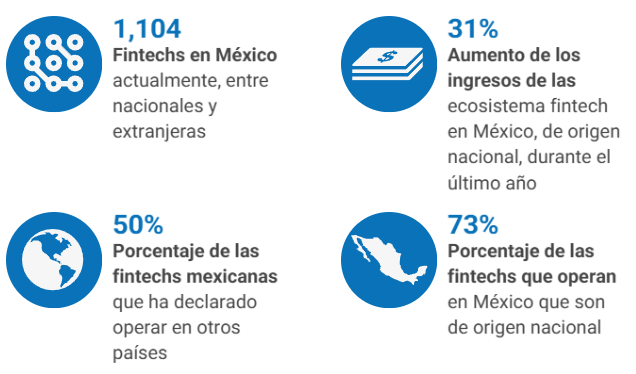
\includegraphics[scale=0.5]{Figuras/datosmercado.png} % scale the figure here
        \captionsetup{labelfont={color=white}, textfont={color=white}} % Cambia el color del caption
        \caption{Datos de Mercado.}
        \label{fig:datmerca}
    \end{subfigure}
    \captionsetup{labelfont={color=white}, textfont={color=white}} % Cambia el color del caption
    \caption{Fuente: Finnovista,  Fintech Radar México, 2025}
    \label{fig:figure1}
\end{figure}


\subsection*{Mercado: Tarjetas y Créditos}
De acuerdo con las bases de datos de la Comisión Nacional Bancaria y de Valores (CNBV)~\cite{cnbv_inclusion_2024}, se construyeron las siguientes tablas que se presentan a continuación.

\begin{table}[h!]
    \centering
    \caption{\textcolor{white}{Número de tarjetas de crédito por tipo de institución (trimestral)}}
    \color{white}
    \begin{tabular}{lcccccc}
        \hline
        \textbf{Institución} & \textbf{2023 T1} & \textbf{2023 T2} & \textbf{2023 T3} & \textbf{2023 T4} & \textbf{2024 T1} & \textbf{2024 T2} \\
        \hline
        Banca Múltiple       &        32,538,425         &        33,380,788         &       34,006,416          &       34,603,588          &        35,110,103         &        35,843,245    \\
        Banca de Desarrollo  &       20,362         &          20,495       &        20,680         &         20,601        &        20,756         &        21,037        \\
        Sofipos              &     3,487,589         &         3,155,757        &        4,011,168         &        3,427,085         &        3,955,533         &        5,194,963      \\
        Socaps               &       4,544          &           6,372      &       9,544          &         13,508        &        17,955         &            22,901     \\
        \hline
    \end{tabular}
    \label{tab:creditos_trimestrales}
\end{table}

\begin{table}[h!]
    \centering
    \caption{\textcolor{white}{Número total de créditos otorgados por tipo de institución (trimestral)}}
    \color{white}
    \begin{tabular}{lcccccc}
        \hline
        \textbf{Institución} & \textbf{2023 T1} & \textbf{2023 T2} & \textbf{2023 T3} & \textbf{2023 T4} & \textbf{2024 T1} & \textbf{2024 T2} \\
        \hline
        Banca Múltiple       &       59,480,857         &        60,704,810         &         61,731,925        &        62,709,348        &         63,108,527        &          64,949,134         \\
        Banca de Desarrollo  &       809,487        &        824,525         &         821,385         &         843,350         &         838,168        &           888,626         \\
        Sofipos              &        3,911,704          &          3,719,181       &         4,677,062          &         4,223,454        &        4,953,483         &           5,852,773       \\
        Socaps               &        2,814,646        &        2,852,568         &        2,861,541         &         2,844,703       &        2,830,927         &           2,898,419       \\
        \hline
    \end{tabular}
    \label{tab:total_creditos_trimestrales}
\end{table}

%% Estaria fino comparar esto contra dinero activo en el mercado i.e. total de dinero en mercado de credito (general; comparar contra \# tarjetas de credito) vs. total de dinero en el mercado de credito (fintech; comparar contra \# tarjetas de fintechs).

\subsection*{Población: Jóvenes $\in[18,30]$}

\subsection*{Población: Económicamente activos}

\subsection*{Hábitos de consumo (México)}

\subsection*{Población: Lineas telefonicas (no prepago)}

\subsection*{Población: Personas que cumplen con req. de ingresos}